
\documentclass[paper=a4, fontsize=11pt]{scrartcl}
\usepackage[T1]{fontenc}
\usepackage{fourier}

\usepackage[english]{babel}												
\usepackage[protrusion=true,expansion=true]{microtype}	
\usepackage{amsmath,amsfonts,amsthm, amssymb} % Math packages
\usepackage[pdftex]{graphicx}	
\usepackage{url}
\usepackage{graphicx}
\usepackage{hyperref}
\usepackage{algpseudocode}
\usepackage{algorithm}
\usepackage{titling}
\usepackage{listings}
\usepackage{xcolor}

\usepackage[immediate]{silence}
\WarningFilter[temp]{latex}{Command} % silence the warning



% Colored Python listing from https://www.overleaf.com/learn/latex/Code_listing
\definecolor{codegreen}{rgb}{0,0.6,0}
\definecolor{codegray}{rgb}{0.5,0.5,0.5}
\definecolor{codepurple}{rgb}{0.58,0,0.82}
\definecolor{backcolour}{rgb}{0.95,0.95,0.92}
 
\lstdefinestyle{mystyle}{
    backgroundcolor=\color{backcolour},   
    commentstyle=\color{codegreen},
    keywordstyle=\color{magenta},
    numberstyle=\tiny\color{codegray},
    stringstyle=\color{codepurple},
    basicstyle=\ttfamily\footnotesize,
    breakatwhitespace=false,         
    breaklines=true,                 
    captionpos=b,                    
    keepspaces=true,                 
    numbers=left,                    
    numbersep=5pt,                  
    showspaces=false,                
    showstringspaces=false,
    showtabs=false,                  
    tabsize=2
}
\lstset{style=mystyle}


%%% Custom sectioning
\usepackage{sectsty}
\allsectionsfont{\centering \normalfont\scshape}


%%% Custom headers/footers (fancyhdr package)
\usepackage{fancyhdr}
\pagestyle{fancyplain}
\fancyhead{}											% No page header
\fancyfoot[L]{}											% Empty 
\fancyfoot[C]{}											% Empty
\fancyfoot[R]{\thepage}									% Pagenumbering
\renewcommand{\headrulewidth}{0pt}			% Remove header underlines
\renewcommand{\footrulewidth}{0pt}				% Remove footer underlines
\setlength{\headheight}{13.6pt}


%%% Equation and float numbering
\numberwithin{equation}{section}		% Equationnumbering: section.eq#
\numberwithin{figure}{section}			% Figurenumbering: section.fig#
\numberwithin{table}{section}				% Tablenumbering: section.tab#


%%% Maketitle metadata
\newcommand{\horrule}[1]{\rule{\linewidth}{#1}} 	% Horizontal rule

\title{
		%\vspace{-1in} 	
		\usefont{OT1}{bch}{b}{n}
		\normalfont \normalsize \textsc{CS 412: Algorithms: Design and Analysis} \\ [25pt]
		\horrule{0.5pt} \\[0.4cm]
		\huge Fast Fourier Transform \\
		\horrule{2pt} \\[0.5cm]
}
\author{
		\normalfont 								\normalsize
        Team \textit{random-theory}\\[-3pt]		\normalsize
        \today
}
\date{}


%%% Begin document
\begin{document}
\maketitle

\section{Introduction}
A \href{https://en.wikipedia.org/wiki/Fourier_transform}{Fourier transform} is a mathematical transform that decomposes functions depending on space or time into functions depending on spatial frequency or temporal frequency.

The central question that fourier transform is trying to solve is that if we have a signal, can we decompose it into the pure frequencies that make it up? such that adding up all the invidual decompositions gives us the original signal back. Its just like unmixing some colors that have been mixed together or finding the recipe of a given smoothie. 

It is one of the most powerful tools in digital signal processing and digital image processing that is used for the the frequency analysis of signals. It is used in a wide range of applications, such as signal interpolation, signal smoothing, image filtering, image reconstruction and image compression. In fact any field of physical science that uses sinusoidal signals, will make use of Fourier series and Fourier transforms. 

\subsection{Fourier Transform of a function}
It gives us a unique way of viewing any function as the sum of simple sinusoids. The Fourier Transform of a function $g(t)$ is defined by:
\begin{equation}
G\left( f \right) = \int_{-\infty}^{\infty} g\left(t\right) \operatorname{e}^{-2\pi ift}
\end{equation}
\newline 
In addition, $g$ can be obtained from $G$ via the inverse Fourier Transform:
\begin{equation}
g\left( t \right) = \int_{-\infty}^{\infty} G\left(F\right) \operatorname{e}^{2\pi ift}
\end{equation}

\subsection{Why use Complex Numbers?}
In the time domain, we have our horizontal and vertical axis. If we were to place our samples on the x-axis, then the y-axis would show the amplitude of those samples. Now, if we were to represent the samples in the frequency domain, our samples need to conserve two properties, the amplitude, and the phase; the latter is quite important for various applications of the transform such as data filtering. Complex numbers provide a nice way of storing the phase.



\section{Discrete Fourier Transform}
In Discrete Fourier Transform, we modify the above integral equations to Fourier transform the discrete finite samples. If we take a sample size of $N$, then there will be exactly $N$ values generated after the transform, thus we can say that DFT maps $N$ complex numbers from one domain, say time, to $N$ complex numbers in another domain, say frequency. Finding the discrete sum of the continuous equations above gives us:
\begin{equation} 
    G_k = \sum_{n=0}^{N-1} g_n \cdot e^{ \frac{-i2\pi}{N} \cdot kn }
\end{equation}

\vspace{5mm}

\subsection{Fourier Matrix}

An N-point DFT is expressed as the multiplication $X=Wx$ where $x$ is the original input signal and $W$ is the N-by-N square DFT matrix.

\begin{equation}
    \omega = e^{\frac{-2\pi i}{N}} 
\end{equation}


\begin{equation}   
  x
  = \left( \begin{array}{c}
        x_0 \\
        x_1 \\
        x_2 \\
        \vdots\\
        x_{N-1} 
    \end{array} \right) 
\end{equation}

\vspace{5mm}

\begin{equation}   
  W = \left( \begin{array}{ccccc}
        1 &  1 & 1 & \ldots & 1 \\
        1 & \omega & \omega^2 & \ldots & \omega^{N-1} \\
        1 & \omega^2 & \omega^4 & \ldots & \omega^{2(N-1)} \\
        \vdots&\vdots&\vdots& \ddots &\vdots\\
        1 & \omega^{N-1} & \omega^{2(N-1)} & \ldots & \omega^{(N-1)(N-1)} 
    \end{array} \right) 
\end{equation}

\vspace{5mm}

\begin{equation}   
    DFT(x) = X = x \cdot W
\end{equation}

\newpage
\begin{lstlisting}[language=python, caption= {A python program to compute DFT of a given signal}, captionpos=b]
def compute_dft(x):
    N = len(x)
    X = [0 for _ in range(N)]
    for i in range(N):
        for j in range((N)):
            omega = np.exp(complex(0, -2) * np.pi / N)
            X[i] += x[j] * omega**(i * j)
    return X
\end{lstlisting}



\section{Fast Fourier Transform}
The FFT employs a divide-and-conquer strategy to divide the DFT computation into odd and even parts. These parts are very similar to the original DFT, and we only need to perform half the computation. This would convert our O($n^2$) algorithm to O($m^2$) where m is n/2. As long as m is divisble by 2, we can recursively repeat this till our running time is O($nlogn$). The psuedocode is as follows:
\begin{center}
\begin{figure}[h]
\caption{\href{https://www.youtube.com/watch?v=h7apO7q16V0&t=1345s&ab_channel=Reducible}{Fourier transform psuedocode}}
\centering
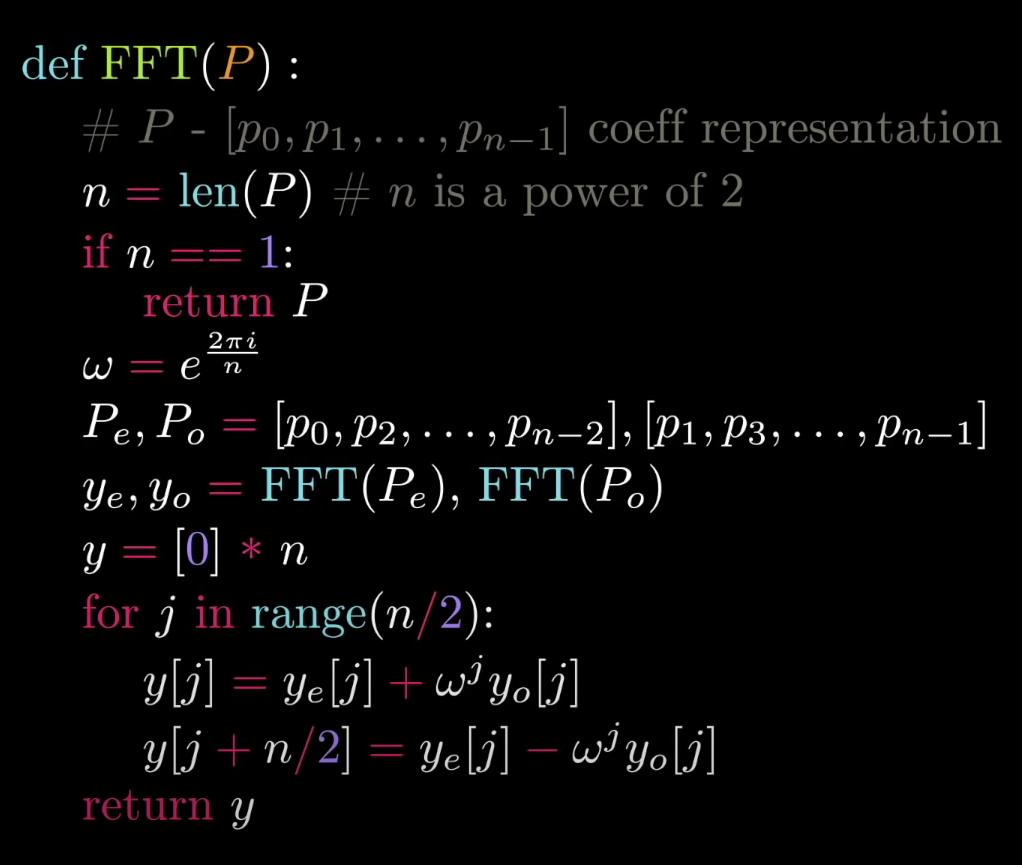
\includegraphics[width=0.7\textwidth]{images/fft.png}
\end{figure}
\end{center}

\vspace{15mm}

\begin{lstlisting}[language=python, caption= {A python program to compute DFT of a given signal using the fast fourier transform}, captionpos=b]
def FFT(X):
    N = len(X)
    if N <= 1: return X
    omega = np.exp(complex(0, -2 * np.pi) / N)

    X_even = FFT(np.array(X[0:N:2]))
    X_odd = FFT(np.array(X[1:N:2]))

    X = [0 for _ in range(N)]

    for j in range(0, N // 2):
        X[j] = X_even[j] + omega**j * X_odd[j]
        X[j + N // 2] = X_even[j] - omega**j * X_odd[j]
    return X
\end{lstlisting}


After recursively dividing the input, P, we only need to run m, or n/2 times. This is what leads to the recurrence of T(n) = 2T(n/2) + O(n). This is only possible because of the symmetric nature of the DFT.

\section{Visualization}

To show the workings of the FFT, we applied it in one of it's most popular applications: signal processing.
We use 2 audio files to show the main functionality the FFT allows.
\begin{itemize}
\item Piano chord being played repeatedly.
\item Background noise while walking in a city.
\end{itemize}
Looking at the first graph below, we see the signal for the piano chord being played repeatedly. We can physically see the chord being repeated in this signal.
In the second graph, we see the signal for the noises in the city. It is more noisy and there are alot more noises mixed in.\\ \\
Essentially, the FFT converts our time domain signal into the frequency domain. It unmixes the frequencies mixed in to the final sound to seperate distinct sounds. In signal processing, this would allow us to identify background noises, or noises to isolate. The FFT identifies the piano chord and we can see this as a peak on the graph. For the second FFT graph, there are alot more noises in the final audio track. These different noises are identified and the most frequent ones are displayed as the highest peaks.


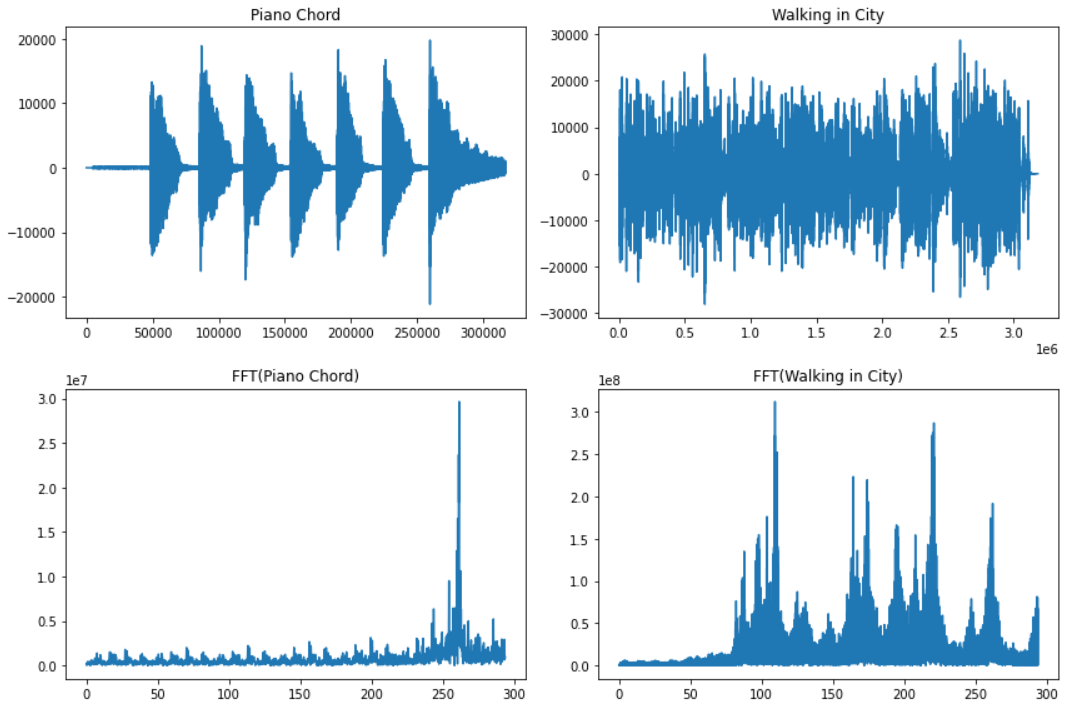
\includegraphics[scale=0.65]{images/fftaudio.png}

\section{Theoretical runtime Analysis}
Lorem ipsum dolor sit amet, consectetuer adipiscing elit. Aenean commodo ligula eget dolor. Aenean massa. Cum sociis natoque penatibus et magnis dis parturient montes, nascetur ridiculus mus. Donec quam felis, ultricies nec, pellentesque eu, pretium quis, sem. In enim justo, rhoncus ut, imperdiet a, venenatis vitae, justo. Nullam dictum felis eu pede mollis pretium. Integer tincidunt. Cras dapibus. Vivamus elementum semper nisi. Aliquam lorem ante, dapibus in, viverra quis, feugiat a, tellus:

Phasellus viverra nulla ut metus varius laoreet. Quisque rutrum. Aenean imperdiet. Etiam ultricies nisi vel augue. Curabitur ullamcorper ultricies 


\section{Experimental runtime Analysis}
Lorem ipsum dolor sit amet, consectetuer adipiscing elit. Aenean commodo ligula eget dolor. Aenean massa. Cum sociis natoque penatibus et magnis dis parturient montes, nascetur ridiculus mus. Donec quam felis, ultricies nec, pellentesque eu, pretium quis, sem. In enim justo, rhoncus ut, imperdiet a, venenatis vitae, justo. Nullam dictum felis eu pede mollis pretium. Integer tincidunt. Cras dapibus. Vivamus elementum semper nisi. Aliquam lorem ante, dapibus in, viverra quis, feugiat a, tellus:

Phasellus viverra nulla ut metus varius laoreet. Quisque rutrum. Aenean imperdiet. Etiam ultricies nisi vel augue. Curabitur ullamcorper ultricies 

\section{Proof of FFT supremacy}
Lorem ipsum dolor sit amet, consectetuer adipiscing elit. Aenean commodo ligula eget dolor. Aenean massa. Cum sociis natoque penatibus et magnis dis parturient montes, nascetur ridiculus mus. Donec quam felis, ultricies nec, pellentesque eu, pretium quis, sem. In enim justo, rhoncus ut, imperdiet a, venenatis vitae, justo. Nullam dictum felis eu pede mollis pretium. Integer tincidunt. Cras dapibus. Vivamus elementum semper nisi. Aliquam lorem ante, dapibus in, viverra quis, feugiat a, tellus:

Phasellus viverra nulla ut metus varius laoreet. Quisque rutrum. Aenean imperdiet. Etiam ultricies nisi vel augue. Curabitur ullamcorper ultricies 

\section{Conclusion}
Lorem ipsum dolor sit amet, consectetuer adipiscing elit. Aenean commodo ligula eget dolor. Aenean massa. Cum sociis natoque penatibus et magnis dis parturient montes, nascetur ridiculus mus. Donec quam felis, ultricies nec, pellentesque eu, pretium quis, sem. In enim justo, rhoncus ut, imperdiet a, venenatis vitae, justo. Nullam dictum felis eu pede mollis pretium. Integer tincidunt. Cras dapibus. Vivamus elementum semper nisi. Aliquam lorem ante, dapibus in, viverra quis, feugiat a, tellus:

Phasellus viverra nulla ut metus varius laoreet. Quisque rutrum. Aenean imperdiet. Etiam ultricies nisi vel augue. Curabitur ullamcorper ultricies 

% \bibliography{refs}
% \bibliographystyle{apalike}


\end{document}